\chapter{Neliöjuurialgoritmit}

\index{nelizjuurialgoritmi@neliöjuurialgoritmi}

\key{Neliöjuurialgoritmi} on algoritmi,
jonka aikavaativuudessa esiintyy neliöjuuri.
Neliöjuurta voi ajatella ''köyhän miehen logaritmina'':
aikavaativuus $O(\sqrt n)$ on parempi kuin $O(n)$
mutta huonompi kuin $O(\log n)$.
Toisaalta neliöjuurialgoritmit toimivat
käytännössä hyvin ja niiden vakiokertoimet ovat pieniä.

Tarkastellaan esimerkkinä tuttua ongelmaa,
jossa toteutettavana on summakysely taulukkoon.
Halutut operaatiot ovat:

\begin{itemize}
\item muuta kohdassa $x$ olevaa lukua
\item laske välin $[a,b]$ lukujen summa
\end{itemize}

Olemme aiemmin ratkaisseet tehtävän
binääri-indeksipuun ja segmenttipuun avulla,
jolloin kummankin operaation aikavaativuus on $O(\log n)$.
Nyt ratkaisemme tehtävän toisella
tavalla neliöjuurirakennetta käyttäen,
jolloin summan laskenta vie aikaa $O(\sqrt n)$
ja luvun muuttaminen vie aikaa $O(1)$.

Ideana on jakaa taulukko $\sqrt n$-kokoisiin
väleihin niin, että jokaiseen väliin
tallennetaan lukujen summa välillä.
Seuraavassa on esimerkki taulukosta ja
sitä vastaavista $\sqrt n$-väleistä:

\begin{center}
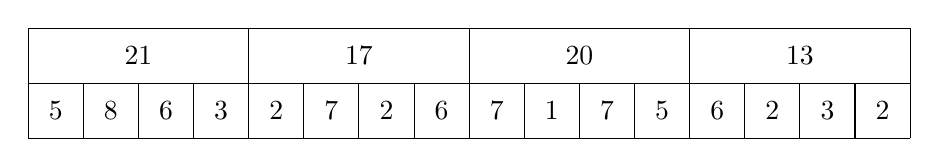
\begin{tikzpicture}[scale=0.7]
\draw (0,0) grid (16,1);

\draw (0,1) rectangle (4,2);
\draw (4,1) rectangle (8,2);
\draw (8,1) rectangle (12,2);
\draw (12,1) rectangle (16,2);

\node at (0.5, 0.5) {5};
\node at (1.5, 0.5) {8};
\node at (2.5, 0.5) {6};
\node at (3.5, 0.5) {3};
\node at (4.5, 0.5) {2};
\node at (5.5, 0.5) {7};
\node at (6.5, 0.5) {2};
\node at (7.5, 0.5) {6};
\node at (8.5, 0.5) {7};
\node at (9.5, 0.5) {1};
\node at (10.5, 0.5) {7};
\node at (11.5, 0.5) {5};
\node at (12.5, 0.5) {6};
\node at (13.5, 0.5) {2};
\node at (14.5, 0.5) {3};
\node at (15.5, 0.5) {2};

\node at (2, 1.5) {21};
\node at (6, 1.5) {17};
\node at (10, 1.5) {20};
\node at (14, 1.5) {13};

\end{tikzpicture}
\end{center}

Kun taulukon luku muuttuu,
tämän yhteydessä täytyy laskea uusi summa
vastaavalle $\sqrt n$-välille:

\begin{center}
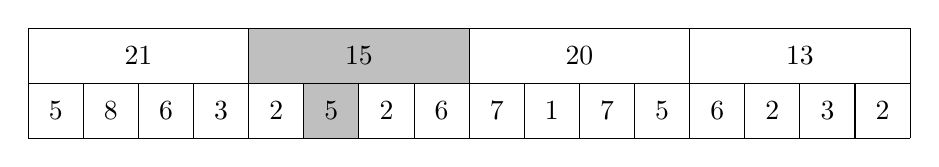
\begin{tikzpicture}[scale=0.7]
\fill[color=lightgray] (5,0) rectangle (6,1);
\draw (0,0) grid (16,1);

\fill[color=lightgray] (4,1) rectangle (8,2);
\draw (0,1) rectangle (4,2);
\draw (4,1) rectangle (8,2);
\draw (8,1) rectangle (12,2);
\draw (12,1) rectangle (16,2);

\node at (0.5, 0.5) {5};
\node at (1.5, 0.5) {8};
\node at (2.5, 0.5) {6};
\node at (3.5, 0.5) {3};
\node at (4.5, 0.5) {2};
\node at (5.5, 0.5) {5};
\node at (6.5, 0.5) {2};
\node at (7.5, 0.5) {6};
\node at (8.5, 0.5) {7};
\node at (9.5, 0.5) {1};
\node at (10.5, 0.5) {7};
\node at (11.5, 0.5) {5};
\node at (12.5, 0.5) {6};
\node at (13.5, 0.5) {2};
\node at (14.5, 0.5) {3};
\node at (15.5, 0.5) {2};

\node at (2, 1.5) {21};
\node at (6, 1.5) {15};
\node at (10, 1.5) {20};
\node at (14, 1.5) {13};

\end{tikzpicture}
\end{center}

Välin summan laskeminen taas tapahtuu muodostamalla
summa reunoissa olevista yksittäisistä luvuista
sekä keskellä olevista $\sqrt n$-väleistä:

\begin{center}
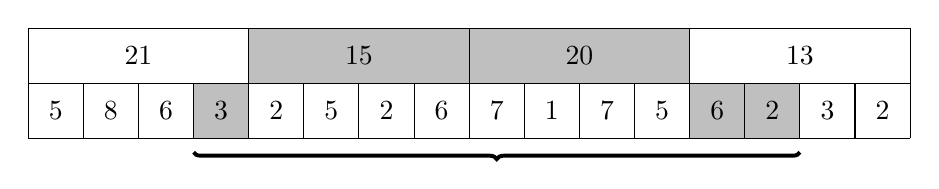
\begin{tikzpicture}[scale=0.7]
\fill[color=lightgray] (3,0) rectangle (4,1);
\fill[color=lightgray] (12,0) rectangle (13,1);
\fill[color=lightgray] (13,0) rectangle (14,1);
\draw (0,0) grid (16,1);

\fill[color=lightgray] (4,1) rectangle (8,2);
\fill[color=lightgray] (8,1) rectangle (12,2);
\draw (0,1) rectangle (4,2);
\draw (4,1) rectangle (8,2);
\draw (8,1) rectangle (12,2);
\draw (12,1) rectangle (16,2);

\node at (0.5, 0.5) {5};
\node at (1.5, 0.5) {8};
\node at (2.5, 0.5) {6};
\node at (3.5, 0.5) {3};
\node at (4.5, 0.5) {2};
\node at (5.5, 0.5) {5};
\node at (6.5, 0.5) {2};
\node at (7.5, 0.5) {6};
\node at (8.5, 0.5) {7};
\node at (9.5, 0.5) {1};
\node at (10.5, 0.5) {7};
\node at (11.5, 0.5) {5};
\node at (12.5, 0.5) {6};
\node at (13.5, 0.5) {2};
\node at (14.5, 0.5) {3};
\node at (15.5, 0.5) {2};

\node at (2, 1.5) {21};
\node at (6, 1.5) {15};
\node at (10, 1.5) {20};
\node at (14, 1.5) {13};

\draw [decoration={brace}, decorate, line width=0.5mm] (14,-0.25) -- (3,-0.25);

\end{tikzpicture}
\end{center}

Luvun muuttamisen aikavaativuus on
$O(1)$, koska riittää muuttaa yhden $\sqrt n$-välin summaa.
Välin summa taas lasketaan kolmessa osassa:

\begin{itemize}
\item vasemmassa reunassa on $O(\sqrt n)$ yksittäistä lukua
\item keskellä on $O(\sqrt n)$ peräkkäistä $\sqrt n$-väliä
\item oikeassa reunassa on $O(\sqrt n)$ yksittäistä lukua
\end{itemize}

Jokaisen osan summan laskeminen vie aikaa $O(\sqrt n)$,
joten summan laskemisen aikavaativuus on yhteensä $O(\sqrt n)$.

Neliöjuurialgoritmeissa parametri $\sqrt n$
johtuu siitä, että se saattaa kaksi asiaa tasapainoon:
esimerkiksi $n$ alkion taulukko jakautuu
$\sqrt n$ osaan, joista jokaisessa on $\sqrt n$ alkiota.
Käytännössä algoritmeissa
ei ole kuitenkaan pakko käyttää
tarkalleen parametria $\sqrt n$,
vaan voi olla parempi valita toiseksi
parametriksi $k$ ja toiseksi $n/k$,
missä $k$ on pienempi tai suurempi kuin $\sqrt n$.

Paras parametri selviää usein kokeilemalla
ja riippuu tehtävästä ja syötteestä.
Esimerkiksi jos taulukkoa käsittelevä algoritmi
käy usein läpi välit mutta harvoin välin sisällä
olevia alkioita, taulukko voi olla järkevää
jakaa $k < \sqrt n$ väliin,
joista jokaisella on $n/k > \sqrt n$ alkiota.

\section{Eräkäsittely}

\index{erxkxsittely@eräkäsittely}

\key{Eräkäsittelyssä} algoritmin suorittamat
operaatiot jaetaan eriin,
jotka käsitellään omina kokonaisuuksina.
Erien välissä tehdään yksittäinen työläs toimenpide,
joka auttaa tulevien operaatioiden käsittelyä.

Neliöjuurialgoritmi syntyy, kun $n$ operaatiota
jaetaan $O(\sqrt n)$-kokoisiin eriin,
jolloin sekä eriä että operaatioita kunkin erän
sisällä on $O(\sqrt n)$.
Tämä tasapainottaa sitä, miten usein erien välinen
työläs toimenpide tapahtuu sekä miten paljon työtä
erän sisällä täytyy tehdä.

Tarkastellaan esimerkkinä tehtävää, jossa
ruudukossa on $k \times k$ ruutua,
jotka ovat aluksi valkoisia.
Tehtävänä on suorittaa ruudukkoon
$n$ operaatiota,
joista jokainen on jompikumpi seuraavista:
\begin{itemize}
\item
väritä ruutu $(y,x)$ mustaksi
\item
etsi ruudusta $(y,x)$ lähin
musta ruutu, kun
ruutujen $(y_1,x_1)$ ja $(y_2,x_2)$
etäisyys on $|y_1-y_2|+|x_1-x_2|$
\end{itemize}

Ratkaisuna on jakaa operaatiot $O(\sqrt n)$ erään,
joista jokaisessa on $O(\sqrt n)$ operaatiota.
Kunkin erän alussa jokaiseen ruudukon ruutuun
lasketaan pienin etäisyys mustaan ruutuun.
Tämä onnistuu ajassa $O(k^2)$ leveyshaun avulla.

Kunkin erän käsittelyssä pidetään yllä listaa ruuduista,
jotka on muutettu mustaksi tässä erässä.
Nyt etäisyys ruudusta lähimpään mustaan ruutuun
on joko erän alussa laskettu etäisyys tai sitten
etäisyys johonkin listassa olevaan tämän erän aikana mustaksi
muutettuun ruutuun.

Algoritmi vie aikaa $O((k^2+n) \sqrt n)$,
koska erien välissä tehdään $O(\sqrt n)$ kertaa
$O(k^2)$-aikainen läpikäynti, ja
erissä käsitellään yhteensä $O(n)$ solmua,
joista jokaisen kohdalla käydään läpi
$O(\sqrt n)$ solmua listasta.

Jos algoritmi tekisi leveyshaun jokaiselle operaatiolle,
aikavaativuus olisi $O(k^2 n)$.
Jos taas algoritmi kävisi kaikki muutetut ruudut läpi
jokaisen operaation kohdalla,
aikavaativuus olisi $O(n^2)$.
Neliöjuurialgoritmi yhdistää nämä aikavaativuudet
ja muuttaa kertoimen $n$ kertoimeksi $\sqrt n$.

\section{Tapauskäsittely}

\index{tapauskxsittely@tapauskäsittely}

\key{Tapauskäsittelyssä} algoritmissa on useita
toimintatapoja, jotka aktivoituvat syötteen
ominaisuuksista riippuen.
Tyypillisesti yksi algoritmin osa on tehokas
pienellä parametrilla
ja toinen osa on tehokas suurella parametrilla,
ja sopiva jakokohta kulkee suunnilleen arvon $\sqrt n$ kohdalla.

Tarkastellaan esimerkkinä tehtävää, jossa
puussa on $n$ solmua, joista jokaisella on tietty väri.
Tavoitteena on etsiä puusta kaksi solmua,
jotka ovat samanvärisiä ja mahdollisimman
kaukana toisistaan.

Tehtävän voi ratkaista
käymällä läpi värit yksi kerrallaan ja
etsimällä kullekin värille kaksi solmua, jotka ovat
mahdollisimman kaukana toisistaan.
Tietyllä värillä algoritmin toiminta riippuu siitä,
montako kyseisen väristä solmua puussa on.
Oletetaan nyt, että käsittelyssä on väri $x$
ja puussa on $c$ solmua, joiden väri on $x$.
Tapaukset ovat seuraavat:

\subsubsection*{Tapaus 1: $c \le \sqrt n$}

Jos $x$-värisiä solmuja on vähän,
käydään läpi kaikki $x$-väristen solmujen parit
ja valitaan pari, jonka etäisyys on suurin.
Jokaisesta solmusta täytyy
laskea etäisyys $O(\sqrt n)$ muuhun solmuun (ks. luku 18.3),
joten kaikkien tapaukseen 1 osuvien solmujen
käsittely vie aikaa yhteensä $O(n \sqrt n)$.

\subsubsection*{Tapaus 2: $c > \sqrt n$}

Jos $x$-värisiä solmuja on paljon,
käydään koko puu läpi ja
lasketaan suurin etäisyys kahden
$x$-värisen solmun välillä.
Läpikäynnin aikavaativuus on $O(n)$,
ja tapaus 2 aktivoituu korkeintaan $O(\sqrt n)$
värille, joten tapauksen 2 solmut 
tuottavat aikavaativuuden $O(n \sqrt n)$.\\\\
\noindent
Algoritmin kokonaisaikavaativuus on $O(n \sqrt n)$,
koska sekä tapaus 1 että tapaus 2 vievät aikaa
yhteensä $O(n \sqrt n)$.

\section{Mo'n algoritmi}

\index{Mo'n algoritmi}

\key{Mo'n algoritmi} soveltuu tehtäviin,
joissa taulukkoon tehdään välikyselyitä ja
taulukon sisältö kaikissa kyselyissä on sama.
Algoritmi järjestää
kyselyt uudestaan niin,
että niiden käsittely on tehokasta.

Algoritmi pitää yllä taulukon väliä,
jolle on laskettu kyselyn vastaus.
Kyselystä toiseen siirryttäessä algoritmi
muuttaa väliä askel kerrallaan niin,
että vastaus uuteen kyselyyn saadaan laskettua.
Algoritmin aikavaativuus on $O(n \sqrt n f(n))$,
kun kyselyitä on $n$ ja 
yksi välin muutosaskel vie aikaa $f(n)$.

Algoritmin toiminta perustuu järjestykseen,
jossa kyselyt käsitellään.
Kun kyselyjen välit ovat muotoa $[a,b]$,
algoritmi järjestää ne ensisijaisesti arvon
$\lfloor a/\sqrt n \rfloor$ mukaan ja toissijaisesti arvon $b$ mukaan.
Algoritmi suorittaa siis peräkkäin kaikki kyselyt,
joiden alkukohta on tietyllä $\sqrt n$-välillä.

Osoittautuu, että tämän järjestyksen ansiosta
algoritmi tekee yhteensä vain $O(n \sqrt n)$ muutosaskelta.
Tämä johtuu siitä, että välin vasen reuna liikkuu
$n$ kertaa $O(\sqrt n)$ askelta,
kun taas välin oikea reuna liikkuu $\sqrt n$
kertaa $O(n)$ askelta. Molemmat reunat liikkuvat
siis yhteensä $O(n \sqrt n)$ askelta.

\subsubsection*{Esimerkki}

Tarkastellaan esimerkkinä tehtävää,
jossa annettuna on joukko välejä taulukossa
ja  tehtävänä on selvittää kullekin välille,
montako eri lukua taulukossa on kyseisellä välillä.

Mo'n algoritmissa kyselyt järjestetään aina samalla
tavalla, ja tehtävästä riippuva osa on,
miten kyselyn vastausta pidetään yllä.
Tässä tehtävässä luonteva tapa on
pitää muistissa kyselyn vastausta sekä
taulukkoa \texttt{c}, jossa $\texttt{c}[x]$
on alkion $x$ lukumäärä aktiivisella välillä.

Kyselystä toiseen siirryttäessä taulukon aktiivinen
väli muuttuu. Esimerkiksi jos nykyinen kysely koskee väliä

\begin{center}
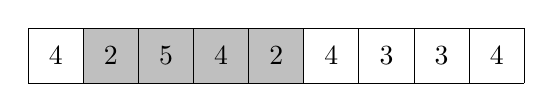
\begin{tikzpicture}[scale=0.7]
\fill[color=lightgray] (1,0) rectangle (5,1);
\draw (0,0) grid (9,1);
\node at (0.5, 0.5) {4};
\node at (1.5, 0.5) {2};
\node at (2.5, 0.5) {5};
\node at (3.5, 0.5) {4};
\node at (4.5, 0.5) {2};
\node at (5.5, 0.5) {4};
\node at (6.5, 0.5) {3};
\node at (7.5, 0.5) {3};
\node at (8.5, 0.5) {4};
\end{tikzpicture}
\end{center}
ja seuraava kysely koskee väliä
\begin{center}
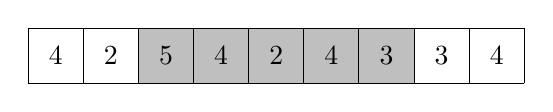
\begin{tikzpicture}[scale=0.7]
\fill[color=lightgray] (2,0) rectangle (7,1);
\draw (0,0) grid (9,1);
\node at (0.5, 0.5) {4};
\node at (1.5, 0.5) {2};
\node at (2.5, 0.5) {5};
\node at (3.5, 0.5) {4};
\node at (4.5, 0.5) {2};
\node at (5.5, 0.5) {4};
\node at (6.5, 0.5) {3};
\node at (7.5, 0.5) {3};
\node at (8.5, 0.5) {4};
\end{tikzpicture}
\end{center}
niin tapahtuu kolme muutosaskelta:
välin vasen reuna siirtyy askeleen oikealle
ja välin oikea reuna siirtyy kaksi askelta oikealle.

Jokaisen muutosaskeleen jälkeen täytyy
päivittää taulukkoa \texttt{c}.
Jos väliin tulee alkio $x$,
arvo $\texttt{c}[x]$ kasvaa 1:llä,
ja jos välistä poistuu alkio $x$,
arvo $\texttt{c}[x]$ vähenee 1:llä.
Jos lisäyksen jälkeen $\texttt{c}[x]=1$,
kyselyn vastaus kasvaa 1:llä,
ja jos poiston jälkeen $\texttt{c}[x]=0$,
kyselyn vastaus vähenee 1:llä.

Tässä tapauksessa muutosaskeleen aikavaativuus on $O(1)$,
joten algoritmin kokonaisaikavaativuus on $O(n \sqrt n)$.


